\documentclass[supercite]{Experimental_Report}

\title{~~~~~~数据结构实验~~~~~~}
\author{张家豪}
\school{计算机科学与技术学院}
\classnum{CS2104}
\stunum{U202115434}
\instructor{袁凌} % 李平、孙伟平、范晔斌、陈加忠
\date{2021年6月10日}

\usepackage{algorithm, multirow}
\usepackage{algpseudocode}
\usepackage{amsmath}
\usepackage{amsthm}
\usepackage{framed}
\usepackage{mathtools}
\usepackage{subcaption}
\usepackage{xltxtra} %提供了针对XeTeX的改进并且加入了XeTeX的LOGO, 自动调用xunicode宏包(提供Unicode字符宏)
\usepackage{bm}
\usepackage{tikz}
\usepackage{tikzscale}
\usepackage{pgfplots}
\usepackage{listings}
%\usepackage{enumerate}

\lstset{
		columns=fixed,       
		numbers=left,                                        % 在左侧显示行号
		numberstyle=\tiny\color{gray},                       % 设定行号格式
		frame=none,                                          % 不显示背景边框
		backgroundcolor=\color[RGB]{245,245,244},            % 设定背景颜色
		keywordstyle=\color[RGB]{40,40,255},                 % 设定关键字颜色
		numberstyle=\footnotesize\color{darkgray},           
		commentstyle=\it\color[RGB]{0,96,96},                % 设置代码注释的格式
		stringstyle=\rmfamily\slshape\color[RGB]{128,0,0},   % 设置字符串格式
		showstringspaces=false,                              % 不显示字符串中的空格
		language=c++,                                        % 设置语言
	}

\pgfplotsset{compat=1.16}

\newcommand{\cfig}[3]{
  \begin{figure}[htb]
    \centering
    \includegraphics[width=#2\textwidth]{images/#1.tikz}
    \caption{#3}
    \label{fig:#1}
  \end{figure}
}

\newcommand{\sfig}[3]{
  \begin{subfigure}[b]{#2\textwidth}
    \includegraphics[width=\textwidth]{images/#1.tikz}
    \caption{#3}
    \label{fig:#1}
  \end{subfigure}
}

\newcommand{\xfig}[3]{
  \begin{figure}[htb]
    \centering
    #3
    \caption{#2}
    \label{fig:#1}
  \end{figure}
}

\newcommand{\rfig}[1]{\autoref{fig:#1}}
\newcommand{\ralg}[1]{\autoref{alg:#1}}
\newcommand{\rthm}[1]{\autoref{thm:#1}}
\newcommand{\rlem}[1]{\autoref{lem:#1}}
\newcommand{\reqn}[1]{\autoref{eqn:#1}}
\newcommand{\rtbl}[1]{\autoref{tbl:#1}}

\algnewcommand\Null{\textsc{null }}
\algnewcommand\algorithmicinput{\textbf{Input:}}
\algnewcommand\Input{\item[\algorithmicinput]}
\algnewcommand\algorithmicoutput{\textbf{Output:}}
\algnewcommand\Output{\item[\algorithmicoutput]}
\algnewcommand\algorithmicbreak{\textbf{break}}
\algnewcommand\Break{\algorithmicbreak}
\algnewcommand\algorithmiccontinue{\textbf{continue}}
\algnewcommand\Continue{\algorithmiccontinue}
\algnewcommand{\LeftCom}[1]{\State $\triangleright$ #1}

\newtheorem{thm}{定理}[section]
\newtheorem{lem}{引理}[section]

\colorlet{shadecolor}{black!15}

\theoremstyle{definition}
\newtheorem{alg}{算法}[section]

\def\thmautorefname~#1\null{定理~#1~\null}
\def\lemautorefname~#1\null{引理~#1~\null}
\def\algautorefname~#1\null{算法~#1~\null}

\begin{document}

\maketitle

\clearpage

\pagenumbering{Roman}

\tableofcontents[level=3]

\clearpage

\pagenumbering{arabic}

\section{基于顺序存储结构的线性表实现}

\subsection{实验目的}

通过实验达到:

(1)加深对线性表的概念、基本运算的理解;

(2)熟练掌握线性表的逻辑结构与物理结构的关系;

(3)物理结构采用顺序表,熟练掌握顺序表基本运算的实现。

\subsubsection{线性表抽象数据类型}

依据最小完备性和常用性相结合的原则,设计了线性表的数据对象和数据关系,并以函数形式定义了线性表的初始化表、销毁表、清空表、判定空表、求表长和获得元素等12种基本运算,具体运算功能定义如下:

(1)初始化表:

InitList(L):

----初始条件:线性表L不存在;

----操作结果:构造一个空的线性表;

(2)销毁表:

DestroyList(L);

----初始条件:线性表L已存在;

----操作结果:销毁线性表L;

(3)清空表:

ClearList(L);

----初始条件:线性表L已存在;

----操作结果:将L重置为空表;

(4)判定空表:

ListEmpty(L);

----初始条件:线性表L已存在;

----操作结果:若L为空表则返回TRUE,否则返回FALSE;

(5)求表长:

ListLength(L);

----初始条件:线性表已存在;

----操作结果:返回L中数据元素的个数;

(6)获得元素:

GetElem(L,i,e);

----初始条件:线性表已存在,1≤i≤ListLength(L);

----操作结果:用e返回L中第i个数据元素的值;

(7)查找元素:

LocateElem(L,e,compare());

----初始条件:线性表已存在;

----操作结果:返回L中第1个与e满足关系compare()关系的数据元素的位序,若这样的数据元素不存在,则返回值为0;

(8)获得前驱:

PriorElem(L,cur\_e,pre\_e);

----初始条件:线性表L已存在;

----操作结果:若cur\_e是L的数据元素,且不是第一个,则用pre\_e返回它的前驱,否则操作失败,pre\_e无定义;

(9)获得后继:

NextElem(L,cur\_e,next\_e);

----初始条件:线性表L已存在;

----操作结果:若cur\_e是L的数据元素,且不是最后一个,则用next\_e返回它的后继,否则操作失败,next\_e无定义;

(10)插入元素:

ListInsert(L,i,e);

----初始条件:线性表L已存在,1≤i≤ListLength(L)+1;

----操作结果:在L的第i个位置之前插入新的数据元素e。

(11)删除元素:

ListDelete(L,i,e);

----初始条件:线性表L已存在且非空,1≤i≤ListLength(L);

----操作结果:删除L的第i个数据元素,用e返回其值;

(13)遍历表:

ListTraverse(L,visit()),

----初始条件:线性表L已存在;

----操作结果:依次对L的每个数据元素调用函数visit()。

附加功能:

(1)最大连续子数组和:

MaxSubArray(L); 

----初始条件:线性表L已存在且非空,请找出一个具有最大和的连续子数组(子数组最少包含一个元素),

----操作结果:其最大和;

(2)和为K的子数组:

SubArrayNum(L,k); 

----初始条件:线性表L已存在且非空, 

----操作结果:该数组中和为k的连续子数组的个数;

(3)顺序表排序:

sortList(L);

----初始条件:线性表L已存在;

----操作结果:将L由小到大排序;

\subsubsection{线性表的文件形式保存}

1.设计文件数据记录格式,以高效保存线性表数据逻辑结构(D,{R})的完整信息;

2.设计了线性表文件保存和加载操作的合理模式。附录B提供了文件存取的具体方法。

\subsubsection{实现多个线性表管理}

在整个链表之外设计包装链表,将已经存在的所有线性表用链式结构串起,对每个线性表赋予独特ID标识,在每次操作中通过ID选择要进行操作的链表。

\subsection{系统设计}

\subsubsection{数据结构设计}

1.线性表的存储数据结构

结构体定义如下:

\begin{lstlisting}
typedef struct
{ //顺序表(顺序结构)的定义
  ElemType *elem;
  int length;
  int listsize;
} SqList;
\end{lstlisting}

2.多线性表的存储数据结构

结构体定义如下:

\begin{lstlisting}
typedef struct
{ //线性表的集合类型定义
  struct
  {
    char name[30];
    SqList L;
  } elem[10];
  int length;
} LISTS;

\end{lstlisting}

在本程序中,数据原子类型被定义为整型int。

\subsubsection{演示系统设计}

包括用户操作界面和功能调用两个部分。

演示系统语言为英文,所有操作和提示语言均为中文。

用户操作界面输出可选的线性表操作,用户输入数字选择要进行的操作。系统提示用户输入参数。

功能调用部分则将用户输入的有关信息传递给线性数据结构的操作函数进行调用,并对函数返回值进行处理判断输出相应提示信息。

\subsection{系统实现}

\subsubsection{线性表运算算法实现}

1.status InitList(SqList \&L);

\textbf{功能: }初始化线性表。

\textbf{算法实现: }为线性表L的data申请空间,申请失败返回ERROR,否则返回成功。

\textbf{时空效率: }时间复杂度为O(1),空间复杂度为O(1)。\\

2.status DestroyList(SqList \&L);

\textbf{功能: }销毁线性表。

\textbf{算法实现: }如果线性表L存在,free掉data空间并设置为null,将其他字段设置为0,返回OK,否则返回INFEASIBLE。

\textbf{时空效率: }时间复杂度为O(1),空间复杂度为O(1)。\\

3.status ClearList(SqList \&L);

\textbf{功能: }清空线性表。

\textbf{算法实现: }如果线性表L存在,将data区域占有的内存空间释放并分配新内存空间,返回OK,否则返回INFEASIBLE。

\textbf{时空效率: }时间复杂度为O(1),空间复杂度为O(1)。\\

4.status ListEmpty(SqList L);

\textbf{功能: }线性表判空。

\textbf{算法实现: }如果线性表L存在,判断L.length是否为0,空就返回TRUE,否则返回FALSE;如果线性表L不存在,返回INFEASIBLE。

\textbf{时空效率: }时间复杂度为O(1),空间复杂度为O(1)。\\

5.status ListLength(SqList L);

\textbf{功能: }获得线性表长度。

\textbf{算法实现: }如果线性表L存在,返回线性表L.length,否则返回INFEASIBLE。

\textbf{时空效率: }时间复杂度为O(1),空间复杂度为O(1)。\\

6.status GetElem(SqList L, int i, ElemType \&e);

\textbf{功能: }获得线性表指定位置数据。

\textbf{算法实现: }如果线性表L不存在,返回INFEASIBLE。如果i不在1与L.length之间,返回ERROR。若上述情况未出现就把L.elem[i-1]的值赋给e,返回ok。

\textbf{时空效率: }时间复杂度为O(n),空间复杂度为O(1)。\\

7.status LocateElem(SqList L, ElemType e); //简化过

\textbf{功能: }寻找指定元素在线性表中位置。

\textbf{算法实现: }如果线性表L存在,遍历线性表数据,若发现数据与e相等就返回index+1;如果e不存在,返回0;当线性表L不存在时,返回INFEASIBLE(即-1)。

\textbf{时空效率: }时间复杂度为O(n),空间复杂度为O(1)。\\

8.status PriorElem(SqList L, ElemType i, ElemType \&pre\_e);

\textbf{功能: }获得指定元素之前的一个元素。

\textbf{算法实现: }如果线性表L存在,遍历查找该元素,将元素前一个位置元素赋值给pre\_e,返回OK;如果没有前驱,返回ERROR;如果线性表L不存在,返回INFEASIBLE。

\textbf{时空效率: }时间复杂度为O(n),空间复杂度为O(1)。\\

9.status NextElem(SqList L, ElemType i, ElemType \&next\_e);

\textbf{功能: }获得指定元素之后的一个元素。

\textbf{算法实现: }如果线性表L存在,遍历查找该元素,将元素前一个位置元素赋值给next\_e,返回OK;如果没有后继,返回ERROR;如果线性表L不存在,返回INFEASIBLE。

\textbf{时空效率: }时间复杂度为O(n),空间复杂度为O(1)。\\

10.status ListInsert(SqList \&L, int i, ElemType e);

\textbf{功能: }插入元素。

\textbf{算法实现: }如果线性表L存在,判断线性表要插入位置是否在1和L.length之间,不是则返回ERROR,判断线性表L.length是否等于L.listsize,相同则空间已满,分配新内存空间;将制定位置后的元素全部后移一个位置,新位置插入在指定位置,返回OK;如果线性表L不存在,返回INFEASIBLE。

\textbf{时空效率: }时间复杂度为O(n),空间复杂度为O(1)。\\

11.status ListDelete(SqList \&L, int i, ElemType \&e);

\textbf{功能: }删除元素。

\textbf{算法实现: }如果线性表L存在,判断线性表要插入位置是否在1和L.length之间,不是则返回ERROR,把L.elem[i-1]的值赋给e,将之后的元素全部前移一个位置,返回OK;当删除位置不正确时,返回ERROR;如果线性表L不存在,返回INFEASIBLE。

\textbf{时空效率: }时间复杂度为O(n),空间复杂度为O(1)。\\

12.status ListTraverse(SqList L);

\textbf{功能: }遍历并打印线性表。

\textbf{算法实现: }如果线性表L存在,直接遍历并打印线性表的所有元素,返回OK;如果线性表L不存在,返回INFEASIBLE。

\textbf{时空效率: }时间复杂度为O(n),空间复杂度为O(1)。\\

\subsubsection{文件存储实现算法}

1.status SaveList(SqList L, char FileName[]);

\textbf{功能: }数据保存。

\textbf{算法实现: }如果线性表L存在,打开文件,根据L.length的大小存入L.elem数据,关闭文件,返回OK;如果线性表L不存在,返回INFEASIBLE。

\textbf{时空效率: }时间复杂度为O(n),空间复杂度为O(n)。\\

2.status LoadList(SqList \&L, char FileName[]);

\textbf{功能: }读取文件。

\textbf{算法实现: }如果线性表L存在,初始化线性表,打开文件,读取数据直到所有数据已经被放入线性表中,根据读取数据的大小改变L.length的值,关闭文件,返回OK;如果线性表L不存在,返回INFEASIBLE。

\textbf{时空效率: }时间复杂度为O(n),空间复杂度为O(n)。\\

\subsubsection{多线性表存储实现算法}

1.status AddList(LISTS \&Lists, char ListName[]);

\textbf{功能: }在多线性表集合里添加线性表。

\textbf{算法实现: }检查过多线性表长度足够后,往多线性表里多申请一块空间给新的线性表,并把输入的ListName赋给新线性表的名字。

\textbf{时空效率: }时间复杂度为O(1),空间复杂度为O(1)。\\

2.status RemoveList(LISTS \&Lists, char ListName[]);

\textbf{功能: }在多线性表集合里删除线性表。

\textbf{算法实现: }遍历多线性表寻找线性表,寻找到后删除线性表并将后面的线性表向前移动一位。

\textbf{时空效率: }时间复杂度为O(n),空间复杂度为O(1)。\\

3.int LocateList(LISTS Lists, char ListName[]);

\textbf{功能: }在多线性表集合里寻找名为ListName的线性表。

\textbf{算法实现: }遍历多线性表寻找线性表,寻找到后返回线性表的逻辑序号。

\textbf{时空效率: }时间复杂度为O(n),空间复杂度为O(1)。\\

\subsection{系统测试}

\subsubsection{实验环境}

实验环境为manjaro linux 5.15.41-1,编译器为gcc版本12.1.0,代码编写使用编辑器VsCode。

文件说明:

def.h:线性表库头文件

function.h:线性表库实现

main.c:演示系统实现

\subsubsection{操作演示}

\begin{figure}[htb]
	\begin{center}
		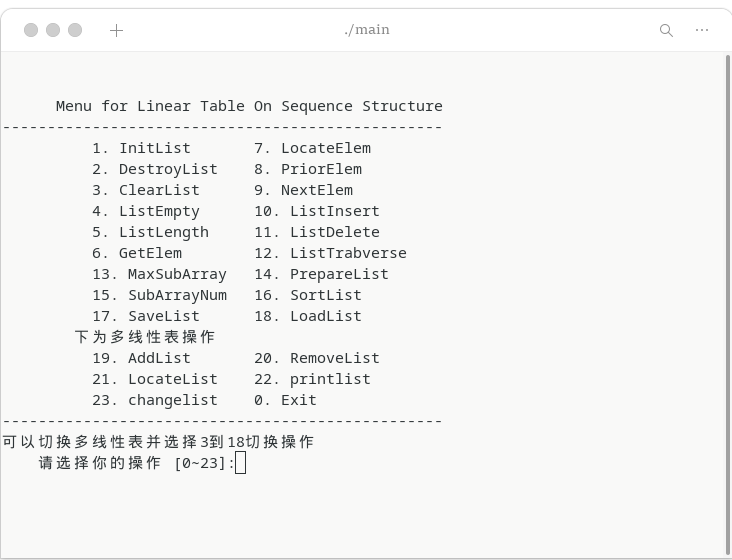
\includegraphics[scale=0.60]{images/1-1.png}
		\caption{系统演示界面}
		\label{fig1-1}
		\end{center}
\end{figure}


\subsection{实验小结}

todo

\newpage

\section{基于邻接表的图实现}

\subsection{实验目的}

通过实验达到

(1)加深对图的概念、基本运算的理解;

(2)熟练掌握图的逻辑结构与物理结构的关系;

(3)以邻接表作为物理结构,熟练掌握图基本运算的实现。

\subsubsection{邻接表抽象数据类型}

依据最小完备性和常用性相结合的原则,以函数形式定义了创建图、销毁图、查找顶点、获得顶点值和顶点赋值等13种基本运算,具体运算功能定义如下。

(1)创建图

CreateCraph(\&G,V,VR);

----初始条件:V是图的顶点集,VR是图的关系集;

----操作结果:按V和VR的定义构造图G。

(2)销毁图:

DestroyBiTree(T);

----初始条件:图G已存在;

----操作结果:销毁图G。

(3)查找顶点

LocateVex(G,u);

----初始条件:图G存在,u和G中的顶点具有相同特征;

----操作结果:若u在图G中存在,返回顶点u的位置信息,否则返回其它信息。

(4)获得顶点值

GetVex (G,v);

----初始条件:图G存在,v是G中的某个顶点;

----操作结果:返回v的值。

(5)顶点赋值

PutVex (G,v,value);

----初始条件:图G存在,v是G中的某个顶点;

----操作结果:对v赋值value。

(6)获得第一邻接点

FirstAdjVex(\&G, v);

----初始条件:图G存在,v是G的一个顶点;

----操作结果:返回v的第一个邻接顶点,如果v没有邻接顶点,返回“空”。

(7)获得下一邻接点

NextAdjVex(\&G, v, w);

----初始条件:图G存在,v是G的一个顶点,w是v的邻接顶点;

----操作结果:返回v的(相对于w)下一个邻接顶点,如果w是最后一个邻接顶点,返回“空”。

(8)插入顶点

InsertVex(\&G,v);

----初始条件:图G存在,v和G中的顶点具有相同特征;

----操作结果:在图G中增加新顶点v。

(9)删除顶点

DeleteVex(\&G,v);

----初始条件:图G存在,v是G的一个顶点;

----操作结果:在图G中删除顶点v和与v相关的弧。

(10)插入弧

InsertArc(\&G,v,w);

----初始条件:图G存在,v、w是G的顶点;

----操作结果:在图G中增加弧<v,w>,如果图G是无向图,还需要增加<w,v>。

(11)删除弧

DeleteArc(\&G,v,w);

----初始条件:图G存在,v、w是G的顶点;

----操作结果:在图G中删除弧<v,w>,如果图G是无向图,还需要删除<w,v>。

(12)深度优先搜索遍历

DFSTraverse(G,visit());

----初始条件:图G存在;

----操作结果:图G进行深度优先搜索遍历,依次对图中的每一个顶点使用函数visit访问一次,且仅访问一次。

(13)广深度优先搜索遍历

BFSTraverse(G,visit());

----初始条件:图G存在;

----操作结果:图G进行广度优先搜索遍历,依次对图中的每一个顶点使用函数visit访问一次,且仅访问一次。

附加功能

(1)距离小于k的顶点集合

VerticesSetLessThank(G,V,K);

----初始条件:图G存在;

----操作结果:返回与顶点v距离小于k的顶点集合;

(2)顶点间最短路径和长度

ShortestPathLength(G,v,w); 

初始条件:图G存在;

操作结果:返回顶点v与顶点w的最短路径的长度;

(3)图的连通分量

ConnectedComponentsNums(G);

初始条件:图G存在;

操作结果:返回图G的所有连通分量的个数;

\subsubsection{邻接表的文件形式管理}

1.设计文件数据记录格式,以高效保存邻接表数据逻辑结构的完整信息;

2.设计了线性表文件保存和加载操作的合理模式。附录B提供了文件存取的具体方法。

\subsubsection{实现多个邻接表管理}

在整个邻接表之外设计包装邻接表,将已经存在的所有邻接表用链式结构串起,对邻接表赋予独特ID标识,通过ID选择要进行操作的链表。

\subsection{系统设计}

\subsubsection{数据结构设计}

1.邻接表的存储数据结构

结构体定义如下:

\begin{lstlisting}
typedef struct
{ //顶点类型定义
  KeyType key;
  char others[20];
} VertexType;

typedef struct ArcNode
{ //表结点类型定义
  int adjvex;              //顶点位置编号
  struct ArcNode *nextarc; //下一个表结点指针
} ArcNode;

typedef struct VNode
{ //头结点及其数组类型定义
  VertexType data;   //顶点信息
  ArcNode *firstarc; //指向第一条弧
} VNode, AdjList[MAX_VERTEX_NUM];

typedef struct
{ //邻接表的类型定义
  AdjList vertices;   //头结点数组
  int vexnum, arcnum; //顶点数、弧数
  GraphKind kind;     //图的类型
} ALGraph;
\end{lstlisting}

2.多邻接表的存储数据结构:

结构体定义如下:

\begin{lstlisting}
typedef struct
{ //邻接表的集合类型定义
  struct
  {
    char name[30];
    ALGraph L;
  } elem[10];
  int length;
} ALGraphs;
\end{lstlisting}

\subsubsection{演示系统设计}

包括用户操作界面和功能调用两个部分。

演示系统语言为英文,所有操作和提示语言均为中文。

用户操作界面输出可选的邻接表操作,用户输入数字选择要进行的操作。系统提示用户输入参数。

功能调用部分则将用户输入的有关信息传递给数据结构的操作函数进行调用,并对函数返回值进行处理判断输出相应提示信息。

\subsection{系统实现}

主要说明各个主要函数的实现思想,复杂函数可辅助流程图进行说明,函数和系统实现的源代码放在附录中。

\subsubsection{邻接表基础运算算法实现}

1.status CreateGraph(ALGraph \&G, VertexType V[], KeyType VR[][2]);

\textbf{功能: }创建图

\textbf{算法实现: }若G不存在,初始化图,用V创建顶点,用VR创建图的边,并遍历寻找顶点后用首插法加入邻接表。

\textbf{时空效率: }时间复杂度为O(n),空间复杂度为O(1)。\\

2.status DestroyGraph(ALGraph \&G);

\textbf{功能: }销毁无向图,删除所有顶点和边。

\textbf{算法实现: }遍历邻接图顶点数据,删除顶点的所有的边后删除顶点。把顶点数和边数设置为0。

\textbf{时空效率: }时间复杂度为O(n),空间复杂度为O(1)。\\

3.int LocateVex(ALGraph G, KeyType u);

\textbf{功能: }寻找指定顶点在邻接表中位置。

\textbf{算法实现: }遍历邻接表顶点,寻找到指定元素则返回其逻辑序号。

\textbf{时空效率: }时间复杂度为O(n),空间复杂度为O(1)。\\

4.status PutVex(ALGraph \&G, KeyType u, VertexType value);

\textbf{功能: }将顶点值修改为value

\textbf{算法实现: }遍历邻接表结点,寻找顶点值为u的结点,将value赋给此结点。

\textbf{时空效率: }时间复杂度为O(n),空间复杂度为O(1)。\\

5.int FirstAdjVex(ALGraph G, KeyType u);

\textbf{功能: }寻找顶点u的第一邻接顶点位序

\textbf{算法实现: }遍历邻接表结点,寻找顶点值为u的结点,返回其第一邻接顶点位序。

\textbf{时空效率: }时间复杂度为O(n),空间复杂度为O(1)。\\

int NextAdjVex(ALGraph G, KeyType v, KeyType w);

\textbf{功能: }寻找顶点w在邻接表顶点v的邻接顶点中下一个邻接顶点位置。

\textbf{算法实现: }遍历邻接表结点,寻找顶点值为u的结点,在其邻接顶点中寻找v,返回v的下一邻接顶点位序后返回OK。

\textbf{时空效率: }时间复杂度为O(n),空间复杂度为O(1)。\\

status InsertVex(ALGraph \&G, VertexType v);

\textbf{功能: }插入顶点。

\textbf{算法实现: }检查已有邻接表中是否存在与v的key相同的顶点,邻接表是否不存在或顶点数大于20,是则返回ERROR,否则在邻接表最后加入v顶点并把该位置的firstarc设置为0,邻接表顶点数加一后返回OK。

\textbf{时空效率: }时间复杂度为O(n),空间复杂度为O(1)。\\

status DeleteVex(ALGraph \&G, KeyType v);

\textbf{功能: }删除顶点及相关的弧。

\textbf{算法实现: }用LocateVex确定v位置并检查合法性,无误则遍历邻接表各顶点删除该顶点及其邻接边数据(每删除一条边则将邻接表总边数减1),将后续顶点前移。再遍历一次邻接表顶点,在每个邻接顶点内对边遍历,若值为v的位置序号则删除该边并将后续边向前移动一次,对边再遍历一次,若值大于v的位置序号则将值-1。将邻接表顶点数减1后返回OK;

\textbf{时空效率: }时间复杂度为O($n^{2}$),空间复杂度为O(1)。\\

status InsertArc(ALGraph \&G, KeyType v, KeyType w);

status DeleteArc(ALGraph \&G, KeyType v, KeyType w);

void DFS(ALGraph \&G, void (*visit)(VertexType), int *k, int i);

status DFSTraverse(ALGraph \&G, void (*visit)(VertexType));

status BFSTraverse(ALGraph \&G, void (*visit)(VertexType));

附加功能:

status VerticesSetLessThank(ALGraph G, KeyType v, int k);

void VerticesSetLess(ALGraph G, ArcNode *p, int k, int *q, int a);

int ShortestPathLength(ALGraph G, KeyType v, KeyType w);

int ConnectedComponentsNums(ALGraph G);

\subsubsection{文件存储算法实现}

status SaveGraph(ALGraph G, char FileName[]);

status LoadGraph(ALGraph \&G, char FileName[]);

\subsubsection{多文件存储算法实现}

status AddGraph(ALGraphs \&Graphs, char GraphName[], VertexType V[], KeyType VR[][2]);

status RemoveGraph(ALGraphs \&Graphs, char GraphName[]);

int LocateGraph(ALGraphs Graphs, char GraphName[]);

\subsection{系统测试}

主要说明针对各个函数正常和异常的测试用例及测试结果

\subsubsection{实验环境}

\subsubsection{操作演示}

\subsection{实验小结}

\newpage

\section{课程的收获和建议}

描述通过学习该专题,有何收获,有何建议,如某专题可适当减少讲授时间、某专题可适当增加讲授内容和时间等。描述通过学习该专题,有何收获,有何建议,如某专题可适当减少讲授时间、某专题可适当增加讲授内容和时间等。描述通过学习该专题,有何收获,有何建议,如某专题可适当减少讲授时间、某专题可适当增加讲授内容和时间等。描述通过学习该专题,有何收获,有何建议,如某专题可适当减少讲授时间、某专题可适当增加讲授内容和时间等。

\subsection{基于顺序存储结构的线性表实现}

描述通过学习计算机基础知识专题,有何收获,有何建议,如某专题可适当减少讲授时间、某专题可适当增加讲授内容和时间等。描述网页的设计和实现过程中遇到的问题及如何解决。描述网页的设计和实现过程中遇到的问题及如何解决。描述网页的设计和实现过程中遇到的问题及如何解决。描述网页的设计和实现过程中遇到的问题及如何解决。描述网页的设计和实现过程中遇到的问题及如何解决。描述网页的设计和实现过程中遇到的问题及如何解决。描述网页的设计和实现过程中遇到的问题及如何解决。描述网页的设计和实现过程中遇到的问题及如何解决。

\subsection{基于链式存储结构的线性表实现}

描述通过学习文档撰写工具LaTeX专题,有何收获,有何建议,如某专题可适当减少讲授时间、某专题可适当增加讲授内容和时间等。描述通过学习文档撰写工具LaTeX专题,有何收获,有何建议,如某专题可适当减少讲授时间、某专题可适当增加讲授内容和时间等。

\subsection{基于二叉链表的二叉树实现}

描述通过学习编程工具Python专题,有何收获,有何建议,如某专题可适当减少讲授时间、某专题可适当增加讲授内容和时间等。描述通过学习编程工具Python专题,有何收获,有何建议,如某专题可适当减少讲授时间、某专题可适当增加讲授内容和时间等。

\subsection{基于二叉链表的二叉树实现}

描述通过学习计算机基础知识专题,有何收获,有何建议,如某专题可适当减少讲授时间、某专题可适当增加讲授内容和时间等。描述通过学习计算机基础知识专题,有何收获,有何建议,如某专题可适当减少讲授时间、某专题可适当增加讲授内容和时间等。


\nocite{*} %% 作用是不对文献进行引用,但可以生成文献列表

\bibliographystyle{Experimental_Report}
\bibliography{Experimental_Report}
\setcounter{secnumdepth}{0}
\appendix

\section{附录A 基于顺序存储结构线性表实现的源程序}

\noindent
/* Linear Table On Sequence Structure */\\
\#include <stdio.h>\\
\#include <malloc.h>\\
\#include <stdlib.h>\\

\noindent
/*---------page 10 on textbook ---------*/\\
\#define TRUE 1\\
\#define FALSE 0\\
\#define OK 1\\
\#define ERROR 0\\
\#define INFEASTABLE -1\\
\#define OVERFLOW -2\\
\newpage
\section{附录B 基于链式存储结构线性表实现的源程序}
\newpage
\section{附录C 基于二叉链表二叉树实现的源程序}
\newpage
\section{附录D 基于邻接表图实现的源程序}

\end{document}